\subsection{ARM Top-Level Software}
The ARM top-level software receives the image data from a remote device and sends the results back to this device. Control of the hardware.

\subsubsection{Requirements}
\todo{Add more information and specify the requirements}
Requirements of the ARM Top-Level Software:
\begin{itemize} 
	\item Receive image data
	\item Also use image data set already stored on device
	\item send results to remote PC
	\item Send and receive control signals from remote PC
	\item Send image data to driver user layer and receive results from driver user layer
	\item Send and receive status and control signals to driver user layer
	\item Run at start-up 
\end{itemize}

\subsubsection{Dynamic Updating of the Bitstream}

Optional feature: Update Bitstream file using \texttt{/dev/xdevcfg}.

Update: For newer versions it looks like \texttt{/dev/xdevcfg} doesn't exist anymore. The problem is discussed here \footnote{\url{https://forum.digilentinc.com/topic/18194-dynamically-load-bitstream-on-petalinux/}} and a potential solution can be found here. \footnote{\url{https://github.com/Digilent/zynq-dynamic-tools}}

\subsubsection{Interface to remote PC}
See Section \ref{subsec:InterfaceRemoteZed}.  
\subsubsection{Interface to kernel layer}
Python wrapper are used for the interface between the top level software which is programmed in python and the hardware drivers which are programmed in C. For usability a high level interface to the underlying C wrapper is made. 
This header interface can then be wrapped to multiple target languages using \cite{Swig2020}. In our case this was done for Python.

\subsubsection{File Tree of ARM Top-Level software} \label{SEC:ARM-TOP-SW-FILE-TREE} \todo{Update this section. Do we still use the C code or do we plan to implement everything in python?}
\begin{figure}[h] 
	\centering
	{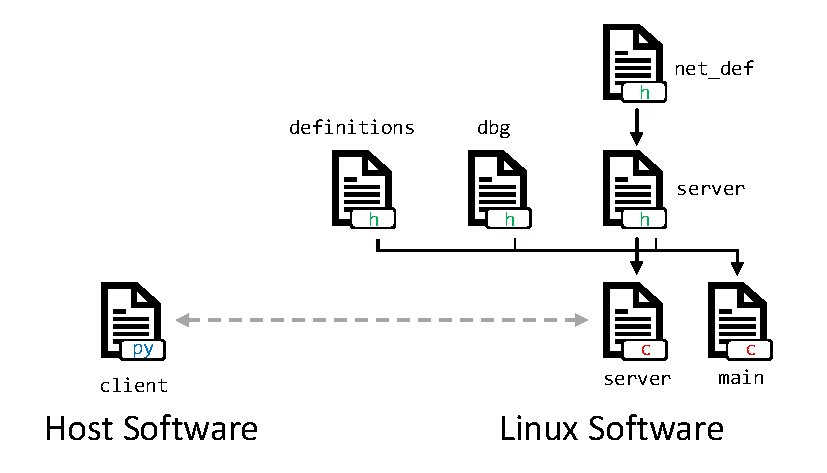
\includegraphics[scale=0.75]{img/software.pdf}} 
	\caption{File tree for the software}
\end{figure} 
\begin{itemize}
	\item \verb|net_def.h| Contains definitions for networking, e.g. ports used.
	\item \verb|dbg.h| Contains debugging macros for logging and error handling.
	\item \verb|definitions.h| Contains information about the neural network, e.g. the number and type of \ac{CNN} stages, layers in the fully connected network, input size and so on.
	\item \verb|server.{c,h}| Handles the connection with the host software.
	\item \verb|main.c| Contains the \verb|main()| function with the main program loop that transmits and manages data to the hardware and from the host system.
	\item \verb|client.py| Handles the connection with the client software.
\end{itemize}
